%! TEX root = icml_drau.tex
\section{Reinforcement learning with a continuous time limit}

In what follows, a discrete algorithm with a well defined time continuous
limit is defined. The algorithm relies on three elements, namely, defining and
learning a quantity that contains some information on the ranking of actions
while admitting a time continuous limit, defining exploration methods that
admit a continuous time limit and defining learning rates that induce well
behaved parameter trajectories when $\deltat$ goes to $0$.

As seen in Sec.~\ref{sec:framework}, there is no continuous time limit to
Q-learning. In continuous time, $Q^\pi$ is independent of actions and can thus
not be used to select promising actions.  In near continuous time, $Q^\pi_\deltat$
still depends on actions, and can still be used to choose promising actions
under the current policy. However, when approximating $Q^\pi_\deltat$, if the
approximation error is much bigger than $\bigO(\deltat)$, approximation errors
dominates, and the ranking of actions given by the approximation is likely to
be erroneous.
% When the approximate Q-function is initialized, if the effect of
% actions on the Q-function is order of magnitudes higher than what it should be,
% approximating $Q^\pi_\deltat$ is likely to be difficult.
%Besides, the error is likely
%to be further propagated when the equation used to update our approximate $Q$
%function relies on bootstraping, as is the case for usual temporal difference
%derived methods.

\subsection{Advantage Updating}
\label{subsec:reparam}
To define an object which contains the same information on actions as
$Q^\pi_\deltat$, but admits an action dependant continuous time limit, it is
natural to define \cite{adv_upd}
\begin{align}
	A^\pi_\deltat(s, a) &\mathdef \frac{Q^\pi_\deltat(s,a) - V^\pi_\deltat(s)}{\deltat},
    \label{eq:adv}
\end{align}
a rescaled version of the advantage function \cite{adv_upd}, as the difference between between
$Q^\pi_\deltat(s, a)$ and $V^\pi\deltat(s)$ is of order $\bigO(\deltat)$.
Contrary to the action state value function, the rescaled advantage function converges when $\deltat$ goes to $0$
to an action dependent quantity which contains the necessary information for policy improvement:


% \LB{In next equation, tiny detail but I would write $\frac{1}{\deltat}(r\deltat+...)$, easier to read.}
% \begin{align}
% 	A^\pi_\deltat(s, a)=&\reward(s, a)+\frac{\gamma^{\deltat}\E_{\delta s \sim \delta s(s, a)}V^\pi_\deltat(s + \delta s)-V^\pi_\deltat(s)}{\deltat}\nonumber\\
% 	=&\reward(s, a)+\log(\gamma) V^\pi(s)+\partial_s V^\pi(s)f(s, a)\nonumber\\
%          &+\frac{\text{tr}\left(\Sigma^T(s, a)\partial^2_{s^2}V^\pi(s) \Sigma(s,a)\right)}{2} + O(\deltat)\nonumber.
% \end{align}

  \begin{theorem}
    There exists $A^\pi(s, a)$ such that for all $a, s$:
    \begin{equation}
      A^\pi_\deltat(s, a) \rightarrow_{\deltat \rightarrow 0} A^\pi(s, a)
    \end{equation}
    Moreover, $A^\pi$ contains all the necessary information for policy improvement. The policy $\pi$ optimal if and only if $A^\pi(s, \pi(s)) = \max_{a'}A^\pi(s, a')$ for all $s \in {\cal S}$.
    \TODO{Is this true? What is true? Is this real life? We should probably add a reasonable hypothesis, for example $\pi_\deltat^* \rightarrow \pi^*$}
  \end{theorem}

The discretized Q-function can be rewritten as
\begin{equation}
	Q^\pi_\deltat(s, a) = V^\pi_\deltat(s) + \deltat A^\pi_\deltat(s, a).
	\label{eq:reparam_q_pi}
\end{equation}
A natural way of approximating $V^\pi_\deltat$ and $A^\pi_\deltat$ is to apply
\emph{Sarsa} or Q-learning to a reparameterized Q-function approximator
\begin{equation}
	Q_\Theta(s, a) = V_{\theta}(s) + \deltat A_{\psi}(s, a).
\end{equation}
with $\Theta = (\theta, \pi)$. To avoid cumbersome notations, in what follows,
parameter indices are dropped.  At initialization, if both $V_{\theta}$ and
$A_{\psi}$ are initialized independantly of $\deltat$, this parameterization
reasonably scales the contribution of actions relative to states in the value
of $Q$.  Our goal is for $V_\theta$ to approximate $V^\pi_\deltat$ and for
$A_{\psi}$ to approximate $A^\pi_\deltat$.


%\TODO{CT and LB are fighting each other about the importance which should be given to the next paragraph. A impartial judge should give his opinion. (CT is wrong)}
However, the proposed reparameterization does not, on its own, guarantee that
when $Q$ correctly approximates $Q^\pi_\deltat$, $A$ approximates $A^\pi_\deltat$\footnote{
	Ensuring that $A$ do not differ from $A^\pi_\deltat$ by a state dependent function only affects
	$A$'s interpretability. Indeed, for any function $f$, the ranking of actions given by
	$A^\pi_\deltat(s, \cdot)$ and $A^\pi_\deltat(s, \cdot) + f(s)$ is the same.
}.
Indeed, for any given pair $V$, $A$,
\begin{align}
	\tilde{V}(s) &= V(s) - f(s)\\
	\tilde{A}(s, a) &= A(s, a) + \frac{f(s)}{\deltat}
\end{align}
yields the exact same $Q$ function. Consequently, $Q$ can correctly approximate
$Q^\pi$ even if $A$ is arbitrarily far from $A^\pi$.
To enforce identifiability of $A$, one must enforce the consistency equation
\begin{equation}
	Q^\pi_\deltat(s, \pi(s)) - V^\pi_\deltat(s) = 0
\end{equation}
on the approximate $A$ and $V$. This translates to
\begin{equation}
	A(s, \pi(s)) = 0.
\end{equation}
With this additional constraint, if $Q = Q^\pi_\deltat$, then $A = A^\pi_\deltat$ and $V = V^\pi_\deltat$.
\begin{align}
	A^\pi_\deltat(s, a) &= \frac{Q^\pi_\deltat(s,a) - V^\pi_\deltat(s)}{\deltat}\\
		    &= \frac{Q(s,a) - Q(s, \pi(s))}{\deltat}\\
		    &= A(s, a).
\end{align}
In the spirit of~\cite{dueling_nets}, this condition is enforced by writing $A$ as
\begin{equation}
\label{eq:Aparam}
	A(s, a) = \bar{A}(s, a) - \bar{A}(s, \pi(s)).
\end{equation}
With this parameterization, one can hope to learn an approximation of $A^\pi_\deltat$,
from which a proper hiearchy of actions can be derived for any $\deltat$.

\subsection{Time invariant exploration}
\label{subsec:explo}
To obtain a time invariant reinforcement learning algorithm, a time invariant
exploration scheme is required. 
\cite{ddpg} already introduces an exploration scheme for continuous actions, which consists in adding an
\emph{Ornstein-Uhlenbeck}~\cite{orn-uhl} process (OU process) to actions, that is naturally time
discretization invariant. Formally, it is defined as
\begin{equation}
	\pi^\text{explore}(s^k_\deltat, z^k_\deltat) = \pi(s^k_\deltat) + z^k_\deltat
\end{equation}
with $z^k_\deltat$ the discretization of a time continuous OU process, defined as
\begin{equation}
	dz_t = - z_t \theta dt + \sigma \dbt.
	\label{eq:orn_uhl}
\end{equation}
where $B_t$ is a brownian motion. Resulting discretized trajectories converge
to non trivial continuous time trajectories.

This exploration can be extended to schemes of the form
\begin{equation}
  \label{eq:explore}
	a^k_\deltat = \pi^\text{explore}_\deltat(s^k_\deltat, z^k_\deltat)
\end{equation}
with $(z^k_\deltat)_k$ a sequence of random variables, independant from the $a$'s and $s$'s.
A sufficient condition for the exploratory policy to admit a time continuous
limit is for
$z_\deltat$ to admit a limit, i.e. that the sequence $z_\deltat$ converges to a
well defined continuous stochastic process $z$ as $\deltat$ goes to $0$.
% For instance, $\varepsilon$-greedy exploration naturally falls in this framework, \TODO{[[CT would like to give these details, LB thinks it is not necessary:]] with each $z^k_\deltat$
% being a pair composed of a bernoulli random variables $b^k_\deltat$ with probability of being $1$ equal to $\varepsilon$,
% and of a uniform categorical random variable $\xi^k_\deltat$ on actions. Exploratory actions are then selected as
% \begin{equation}
% 	a^k_\deltat = (1 - b^k_\deltat) \text{argmax}_{a'} Q^\pi_\deltat(s, a') + b^k_\deltat \xi^k_\deltat.
% \end{equation}}
To obtain a temporally coherent exploration scheme in discrete action environment
$z_\deltat$ is chosen to be a discretization of a $|\mathcal{A}|$ dimensional
continuous OU process, and set
\begin{equation}
  \pi^\text{explore}(s_t, z_t)= \text{argmax}_{a'} \left(Q(s, a') + z_t[a']\right)
\end{equation}
where $z_t[a']$ denotes the $a'$-th component of the discretized OU process at time
$k$. The resulting exploration scheme converges to a proper time continuous exploration scheme,
and is non trivial for most $Q$'s.

Contrary to this discrete action exploration scheme, $\varepsilon$-greedy
exploration is likely to not explore, i.e. to collapse to a deterministic
policy when $\deltat$ goes to $0$. Indeed, one can prove that in a near
continuous deterministic environment, the exploration policy resulting from
applying $\varepsilon$ greedy exploration to a constant exploitation policy
converges to a determinist policy as $\deltat$ goes to $0$. More precisely, let
$(a_\deltat)$ a sequence of i.i.d. actions of distribution $p_A$, (for instance
the sequence of actions generated by $\varepsilon$-greedy exploration on a
constant policy). Then, as $\deltat$ goes to $0$, trajectories generated by
interacting with the environment using the $a$'s converge to solutions of
\begin{equation}
	ds_t = \E_{a\sim p_A}\left[F(s_t, a)\right]dt
\end{equation}
where the expectation cancels the exploration noise. The proof is given in the
supplementary material.

\subsection{Algorithms}
\label{subsec:algorithm}
\begin{algorithm}[ht]
	\caption{Deep Advantage Updating (Discrete actions)}
	%! TEX root = icml_drau.tex
\begin{algorithmic}
	\STATE \textbf{Inputs:}
	\STATE $\theta$ and $\psi$, parameters of
	$V_{\theta}$ and $\bar{A}_{\psi}$.
	\STATE $\pi^{\text{explore}}$ and $\nu_\deltat$ defining an exploration policy.
	\STATE \textbf{opt}$_1$, \textbf{opt}$_2$, $\alpha_1 \deltat$ and $\alpha_2 \deltat$ optimizers and learning rates.
	\STATE $\mathcal{D}$, buffer of transitions $(s, a, r, d, s')$, with $d$ the episode termination signal.
	\STATE $\deltat$ and $\gamma$, time discretization and discount factor.
	\STATE \textbf{nb\_epochs} number of epochs.
	\STATE \textbf{nb\_steps}, number of steps per epoch.
	\STATE
	\STATE Observe initial state $s^0$
	\STATE $t \gets 0$
	\FOR {$e=0, \textbf{nb\_epochs}$}
	\FOR {$j=1, \textbf{nb\_steps}$}
	\STATE $a^k \leftarrow \pi^{\text{explore}}(s^k, \nu^k_\deltat)$.
	\STATE Perform $a^k$ and observe $(r^{k+1}, d^{k+1}, s^{k+1})$.
	\STATE Store $(s^k, a^k, r^{k+1}, d^{k+1}, s^{k+1})$ in $\mathcal{D}$.
	\STATE $k \gets k + 1$
	\ENDFOR
	\FOR {$k=0, \text{nb\_learn}$}
	\STATE \text{Sample a batch of $N$ random transitions from $\mathcal{D}$}
	\STATE $Q^i \gets V_{\theta}(s^i) + \deltat\hspace{-.17em}\left(
	\bar{A}_{\psi}(s^i, a^i) - \max\limits_{a'}\bar{A}_{\psi}(s^i, a')\right)$
	\STATE $\tilde{Q^i} \gets r^i\deltat + (1 - d^i) \gamma^{\deltat} V_{\theta}(s'^i)$
	\STATE $\Delta \theta \gets \frac{1}{N}\sum\limits_{i=1}^N  \frac{\left(Q^i - \tilde{Q^i}\right)\partial_{\theta} V_{\theta}(s^i)}{\deltat}$
	\STATE $\Delta \psi \gets \frac{1}{N}\sum\limits_{i=1}^N \frac{\left(Q^i - \tilde{Q^i}\right)\partial_{\psi} \left(\bar{A}_{\psi}(s^i, a^i) - \max\limits_{a'}\bar{A}_{\psi}(s^i, a')\right) }{\deltat}$
	\STATE Update $\theta$ with \textbf{opt}$_1$, $\Delta \theta$ and learning rate $\alpha_1 \deltat$.
	\STATE Update $\psi$ with \textbf{opt}$_2$, $\Delta \psi$ and learning rate $\alpha_2 \deltat$.
	\ENDFOR
	\ENDFOR
\end{algorithmic}

	\label{alg:dau}
\end{algorithm}

To learn $V_{\theta}$ and $A_{\psi}$, variants of Q-learning for continuous and
discrete action spaces are used. In details, $V_{\theta}$ and $A_{\psi}$ are learnt
using approximate version of the following bellman equation, which holds for the true $A^\pi_\deltat$
and $V^\pi_\deltat$, with a greedy exploitation policy $\pi(s) = \text{argmax}_{a'}A^\pi_\deltat(s, a')$
\begin{align}
	V^{\pi}_\deltat(s) + \deltat A^{\pi}_\deltat(s, a) &= r\deltat + \gamma^{\deltat}  \E_{s'} V^{\pi}_\deltat(s')\label{eq:bellman_A}\\
	A^{\pi}_\deltat(s, \pi(s)) &= 0\label{eq:max_A}.
\end{align}
Maximization over actions is implemented exactly in the discrete actions case,
and approximated by a policy neural network $\pi_\phi(s)$, trained to maximize $A(s,
\pi_\phi(s))$ in the continuous case.  This is similar to what is done in
\cite{ddpg}.

Eq.~\eqref{eq:max_A}
is directly verified by $A_{\psi}$, owing to the reparametrization
$A_\psi(s, a) = \bar{A}_\psi(s, a) - \bar{A}_\psi(s, \pi(s))$, described
in~\ref{subsec:reparam}.  To approximately verify~\eqref{eq:bellman_A}, the
corresponding squared residual is minimized by an approximate gradient descent.
The update equations when learning from a transition $(s, a, r, s')$, either from
an exploratory trajectory or from a replay buffer~\cite{dqn} are
\begin{align}
	\delta Q_\deltat &\leftarrow A(s, a) \deltat - \left(r \deltat + \gamma^{\deltat} V(s') - V(s)\right)\\
	\theta_\deltat &\leftarrow \theta_\deltat + \eta^V_\deltat \partial_{\theta} V(s) \frac{\delta Q_\deltat}{\deltat}\\
	\psi_\deltat &\leftarrow \psi_\deltat + \eta^A_\deltat \partial_{\psi} A(s, a) \frac{\delta Q_\deltat}{\deltat}.
	\label{eq:approx_bellman_A}
\end{align} 
where $\eta$'s are learning rates.
Appropriate scalings for the learning rates $\eta^V_\deltat$ and $\eta^A_\deltat$ in term of $\deltat$ to obtain a well defined continuous limit are derived in the following section.
% As we will see in the following section,
% to obtain a well defined continuous time limit, the learning rates can be rewritten as
% $\eta^i_\deltat = \alpha^i \deltat$, where $\alpha^1$ and $\alpha^2$ are independant
% of $\deltat$.
\subsection{Learning rates scalings}
\label{subsec:lr}
%! TEX root = icml_drau.tex
\newcommand{\iw}{1cm}
\begin{figure*}[ht]
	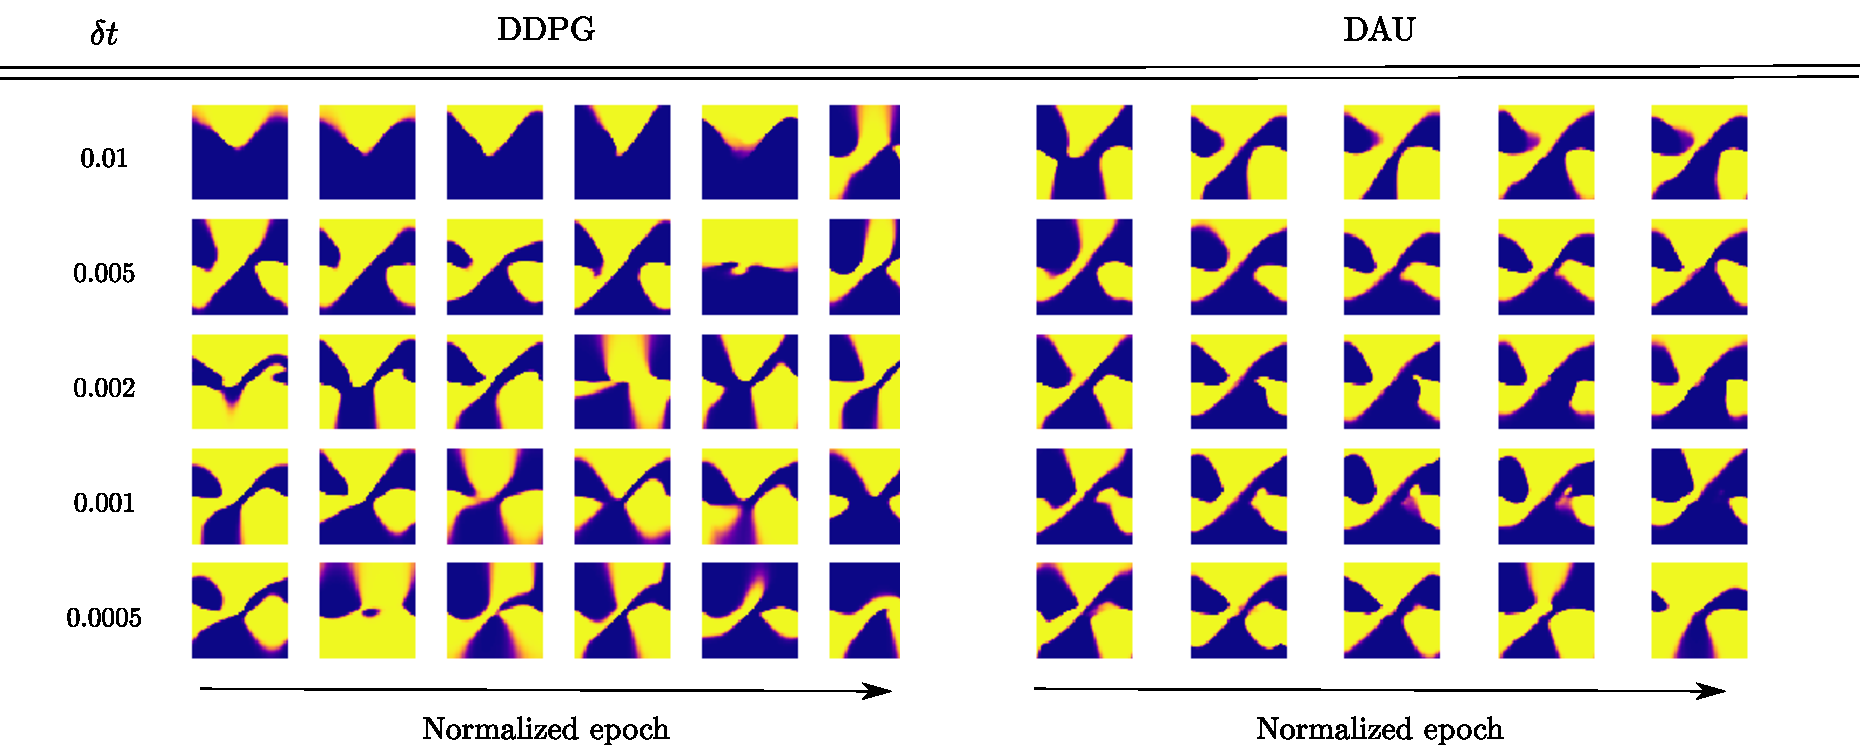
\includegraphics[width=\textwidth]{figs_data/pendulum_fig.pdf}
	\caption{Policies obtained by DDPG and AU at different macroscopic instants of training. Each image represents the policy learnt by the policy network, with $x$-axis representing angle, and $y$-axis angular velocity. The lighter the pixel, the closer to $1$ the action, the darker, the closer to $-1$.}
\end{figure*}

For the discrete algorithm to admit a continuous time limit, the trajectories
of parameters must converge to well defined trajectories as $\deltat$ goes to
$0$.  Intuitively, this means that optimization steps should not be too large,
in which case parameter trajectories could diverge in a single gradient step,
or too small, in which case the trajectories would converge to single points as
$\deltat$ goes to $0$.  This in turn imposes conditions on the scalings of the
learning rates of algorithms robust to changes of the tine discretization.

The updates equations on $\theta$ and $\psi$ are described in
Eq.~\eqref{eq:approx_bellman_A}.  To have parameter steps that do not explode or shrink to $0$ too
fast as $\deltat \rightarrow 0$, both $\delta \theta$ and
$\delta \psi$ should verify stochastic differential equations, and notably
have a deterministic component of order $\deltat$. As $\deltat$ goes to $0$,
updates are rephrased as
\begin{align}
	\delta Q_\deltat &= A(s, a)\deltat - r\deltat - \log(\gamma) V(s)\deltat - \partial_s V(s) \delta s\nonumber \\&- \frac{(\delta s)^T \partial_{s^2}^2 V(s) \delta s}{2} + \smallo\left(\deltat\right)\\
	\delta \theta_\deltat &= \eta^V_\deltat \partial_{\theta} V(s) \frac{\delta Q_\deltat}{\deltat} + \smallo\left(\eta^V_\deltat\right)\\
	\delta \psi_\deltat &= \eta^A_\deltat \partial_{\psi} A(s) \frac{\delta Q_\deltat}{\deltat} + \smallo\left(\eta^A_\deltat\right).
\end{align}


For parameter updates to follow a SDE, one must
have $\eta^V_\deltat = \alpha^V \deltat$ and $\eta^A_\deltat = \alpha^A
\deltat$. More precisely
\begin{theorem}
	\TODO{We need a bit more details: we probably want to assume that states and actions are
	drawn from a single fixed trajectory, and that we are learning for a fixed, constant policy.}
	Let $\eta^V_\deltat = \alpha^V \deltat^\beta$ (resp. $\eta^A \deltat^\beta$) be the learning rate
	of $V$ (resp. $A$), when training on a single exploratory trajectory. Then
	\begin{itemize}
		\item If $\beta = 1$ the discrete parameter trajectories converge to continuous parameter
			trajectories as $\deltat$ goes to $0$.
		\item If $\beta < 1$, parameters grow arbitrarily large in a single timestep as $\deltat$
			goes to $0$.
		\item If $\beta > 1$, parameter trajectories shrink to a single point as 
			$\deltat$ goes to $0$.
	\end{itemize}
	\label{th:cont-params}
\end{theorem}

% With this choice of learning rates, the limit SDEs are
% \begin{align}
% 	F &= A(s_t, a_t) - r_t - \log(\gamma) V(s_t) - \partial_s V(s_t) f(s_t, a_t)\nonumber\\
% 	G &= - \partial_s V(s_t, a_t) \Sigma(s_t, a_t)\nonumber\\
% 	d\theta_t &= (\alpha^V Fdt  + D \dbt)\partial_{\theta} V(s_t)\nonumber\\
% 	d\psi_t &= (\alpha^A Fdt  + D \dbt)\partial_{\psi} A(s_t, a_t)\nonumber.
% \end{align}
The full algorithm can now be derived.
Pseudocode for the discrete actions algorithm is given in Alg.~\ref{alg:dau}.
Pseudocode for the continuous actions algorithm is given in the supplementary
material.
\TODO{Be careful when using RMSprop. When you are facing a stochastic environment
	RMSprop evaluates the second momentum of gradients and rescale gradients by its
	square root. This second momentum will
	be of order $\frac{1}{\deltat}$, due to the stochasticity in the environment. Consequently
	all gradient steps are multiplied by $\sqrt{\deltat}$, and learning rates need only be
multiplied by $\sqrt{\deltat}$ instead of $\deltat$. Taking batches of size proportional to $\frac{1}{\deltat}$
applies a similar fix.}

